\documentclass[a4paper,12pt]{report}
\usepackage[utf8]{inputenc}
\usepackage{fontspec}
\usepackage[ngerman]{babel}
\usepackage[parfill]{parskip}
%\usepackage{eurosans}
\usepackage[top=3cm, left=3cm]{geometry}
\usepackage{setspace}
\usepackage{mdwlist}
\usepackage{graphicx}
\usepackage{eurosym}
\usepackage{pdfpages}
\usepackage{tikzsymbols}
\usetikzlibrary{shapes}
\usepackage{csquotes}
\renewcommand*\familydefault{\sfdefault}

\definecolor{esebgcolor}{rgb}{1, 1, 1} % wip-ish color -- #0D5F98
\definecolor{esefgcolor}{rgb}{0,0,0}

\setcounter{secnumdepth}{-1}
\setcounter{tocdepth}{1}
\begin{document}

\title{\huge{\textbf{Vor dem Tutorium lesen und wichtige Punkte markieren!}}\\\ \\\ \\{Leitfaden für ESE-Tutoren 2019}}
\date{}
\author{}
\maketitle

\section*{Anwesenheit in der ESE}
Eure Anwesenheit ist zu folgenden Zeiten ausdrücklich erforderlich:
\begin{itemize*}
	\item Aufgabenbereiche, in denen ihr explizit als Helfer eingetragen seid
	\item Frühstück, Tütentragen und Begrüßung am Montag
	\item Bunter Nachmittag am Montag
	\item Wanderung am Mittwoch
	\item Einschreibung am Donnerstag
	\item ESE-Spiel am Freitag
	\item Tutorenabschlussgrillen am Samstag 19:00 Uhr % noch nicht festgelegt
\end{itemize*}
Wichtig für die einzelnen Termine sind auch die vorhering Tutorenbriefings im Ratsaal. Diese sind unbedingt zu besuchen und werden bei nicht erscheinen mit dem Nichtmögen von Tutoren geahndet.\\
WICHTIG: Das Briefing am Donnerstagmorgen ist die einzige Möglichkeit als Nicht-Ersti eine ESE Tasse zu erhalten.
Termine für die Briefings sind:
\begin{itemize*}
	\item Montag   		08:00 Uhr
	\item Dienstag 		12:00 Uhr (Mittag bitte vorher essen)
	\item Donnerstag	08:00 Uhr
	\item Freitag		13:00 Uhr (Mittag bitte vorher essen)
\end{itemize*}

Die Anwesenheit zu allen anderen Veranstaltungen ist wünschenswert!

\section*{Aufgaben eines ESE-Tutors}

\begin{itemize*}
    \item \textbf{Proud to be a Tutor:} Trage während der Woche zu allen ESE-Veranstaltungen (auch abends) das ESE-Shirt und dein Namensschild.
    \item \textbf{Präsenz zeigen:} Sei während der ESE so oft wie möglich da, komm zum Frühstück usw.\ mit den Erstis ins Gespräch.
    \item \textbf{Sei Hilfsbereit:} Siehst du einen einsamen Ersti, hilf ihm, Anschluss zu finden. Ein Ersti fragt dich etwas oder ein Ersti guckt sich verloren um? Setze alles daran zu helfen!
\end{itemize*}

\section*{Ansprechpartner}
FSR/ESE-Orga (ese-orga@ifsr.de): 0351/463-38226 \\

Während der ESE-Woche sollte immer ein Orga-Mitglied im Büro sitzen. Wenn ihr Probleme habt, bitte im Büro anrufen.

\tableofcontents
\chapter{Hinweise für Tutoren}
\section{Himmel statt Scheine}
Scheine gibt es nicht mehr. Zur Motivation haben wir dieses Jahr den Himmel. Der Himmel ist im Raum APB/E008 zu finden und soll als Rückzugsort für euch als Tutoren dienen. Dort könnt ihr euch entspannen und gleichzeitig Feedback an der Tafel hinterlassen. Doch so gemütlich es dort sein mag, solltet ihr doch hin und wieder mal nach draußen gehen und Teil der ESE sein.

\section{Über das Tutorium}
Ziel des Tutoriums ist Vermittlung von Informationen rund um das Studium. Der Inhalt des zweiten Teils dieser Handreichung ist das Minimum, was ihr in den Tutorien vermitteln sollt, ihr könnt die Stichpunkte gerne noch mit eigenen Einfällen ergänzen.\\
Beachtet dabei:
\begin{itemize*}
\item Die Informationen sollten möglichst \textbf{unparteiisch} und \textbf{nicht wertend} vermittelt werden.
Insbesondere sollte man vermeiden, den Erstis schon vorab Angst vor bestimmten Vorlesungen oder Dozenten zu machen oder sie zum Nichtbesuchen der Vorlesungen zu animieren. Das betrifft auch das ESE-Spiel.
\item Eine Tutoriengruppe besteht aus zwei Tutoren und ca. 15--25 Erstis.
\item Solltet ihr zu einem der Themen keine Ahnung haben, dann verweist auf den FSR\@.
\end{itemize*}

\section{Vor dem Tutorium zu erledigende Dinge}
\begin{itemize*}
\item Überlegt euch, wie ihr die Informationen vortragen wollt.
\item Den Raum bitte vorher schon mal suchen, falls ihr nicht sicher wisst, wo er sich befindet.
\item Am ESE-Montag zum Briefing um 08:30 da sein und mit helfen!
\end{itemize*}
\label{tabelle}
\begin{center}
\vspace{1cm}
\begin{tabular}[h]{|l|l|}
	\hline
	\textbf{Namenspatron}		& \textbf{Raum}\\ \hline
	Edsger Dijkstra				& BAR/128\\
	Kathleen Antonelli			& BAR/E85\\
	Kurt Gödel					& BAR/I89\\
	Konrad Zuse					& BAR/213\\
	Tim Berners-Lee				& BAR/106\\
	John von Neumann			& GER/51\\
	Dennis Ritchie				& GER/49\\
	Alan Turing 				& GER/50\\
	Ada Lovelace				& GER/09\\
	Grace Hopper				& GER/07\\
	Constanze Kurz				& GER/54\\
	Anna Biselli				& APB/3105\\
	Adele Goldberg				& APB/1096\\
	Linus Torvalds				& APB/E001\\
	Noam Chomsky				& APB/E005\\
	Christiane Floyd			& APB/E006\\
	Stephen Cook				& APB/E007\\
	Ken Thompson				& APB/E008\\
	Donald Knuth				& APB/E009\\
	Margaret Hamilton			& APB/E010\\
	Andreas Pfitzmann			& APB/E023\\
	\hline
\end{tabular}
\end{center}

\chapter{In den Tutorien zu vermittelnde Informationen}

\section{Ablaufplan}
\begin{itemize*}
	\item Einführung
	\item Überblick ESE-Woche
	\item Kennenlernen
	\item Außerhalb vom Studium
	\item Gemeinsam Mensen
\end{itemize*}

\section{Einführung}
\begin{itemize*}
	\item Wenn ihr Master Studierende in eurer Gruppe habt, schickt sie in den APB E023
	\item Fragt für den Spieleabend nach Grillgutestimates. Zur Wahl stehen Steak, Bratwurst (Rind oder Schwein), Grillkäse, Hähnchenfleisch und Veganes (Pommes oder Grillgemüse). 
	\textbf{Wichtig!} Hierbei geht es nicht um das Studium. Versucht deshalb Fragen zum Studiengang zu vermeiden.\\
	Schreibt am besten an die Tafel, was ihr gerne von den Erstis wissen möchtet.
	\item Schreibt eure Emailadressen an die Tafel, für Nachfragen.
	\item Erzählt etwas zu eurem Namenspatron. Informationen findet ihr im Anhang.
\end{itemize*}

\section{Überblick ESE-Woche}
\begin{itemize*}
	\item ESE-Website: https://ese.ifsr.de (mit aktuellem Ablaufplan der ESE-Woche (kurzfristige Änderungen und Ankündigungen werden via Twitter @ifsr verkündet und abschließend auf der ESE-Seite selbst), Weblinks, etc.)
	\item In diesem Jahr lässt sich die ESE-Webseite als PWA ("Progressive Web App" bzw. als Shortcut <https://ese.ifsr.de/2019/pwa/>) auf den Mobilgeräten installieren. Damit hat man direkten Zugriff auf dem ESE Ablaufplan. Ebenfalls gibt's den Zeitplan auch im iCal-Format (ICS Datei) auf ese.ifsr.de zum Download.
	Kann man sich direkt in den Kalender importieren.
	\item Der Ablaufplan der ESE wird am FSR-Büro hinter der Wendeltreppe hängen und auf der ESE-Webseite stehen.
	\item Die wichtigen Dinge der ESE-Tüte durchgehen.
	\item Geht die ESE-Woche durch und sagt kurz etwas zu den wichtigsten Programmpunkten (siehe Zeitplan und folgende Anmerkungen zu den einzelnen Tagen)
	\item Bitte betont nochmal, dass die ESE sehr gut geeignet ist, um Kommilitonen kennenzulernen.
\end{itemize*}
Ort der Begrüßung ist der Hörsaal HSZ/004 (Hörsaal-Zentum) und der der Vorträge ist die ganze Woche über die APB/E023.

% TODO Plan von unten Einfügen und Kommentare auf Seite daneben

\textbf{Montag}
\begin{itemize*}
	\item 08:30 -- 09:45 Frühstück
	\item 10:00 -- 12:30 Begrüßung im HSZ/004 und Tutorien (siehe Tabelle auf S.\pageref{tabelle})
	\item ab 12:30 Mittagspause bis 13:30
	\small{\textit{%
			\begin{itemize*}
				\item Geht zusammen mit euren Erstis in die Mensa!
				\item Mensakarten gibt es immer beim Frühstück oder nachher im FSR-Büro
				\item E-Meal aufladen erklären! Automaten, Infopoint, Autoload, an der Kasse
				\item Am Nachmittag Sprechstunde im FSR-Büro
			\end{itemize*}
	}}
	\item 13:30 -- 15:30 Vorstellung der Lehrenden
	\item 15:30 -- 18:00 Bunter Nachmittag
	\item ab 18:00 Kennenlernspieleabend
\end{itemize*}

\textbf{Dienstag}
\begin{itemize*}
	\item 09:00 -- 09:45 Frühstück
	\item 10:00 -- 12:00 Vorträge zum Studium
	\item 12:00 -- 13:00 Mittagessen
	\item 13:00 -- 16:00 Campusschnitzeljagd
	\item 17:30 -- 19:00 Vorglühen im CountDown
	\small{\textit{%
			\begin{itemize*}
				\item Möglichkeit auf Freigetränke.
			\end{itemize*}
	}}
	\item ab 19:00 Clubwanderung
	\small{\textit{%
			\begin{itemize*}
				\item Startet beim Studentenclub CountDown (Güntzstraße 22)
			\end{itemize*}
	}}
\end{itemize*}

\textbf{Mittwoch}
\begin{itemize*}
	\item Wanderung (parallel zu Katerfrühstück)
	\small{\textit{%
			\begin{itemize*}
				\item Zeit und Treffpunkt: Start am Hauptbahnhof, Gleis 18, 09:00 Uhr
				\item Bitte Interesse erfragen
			\end{itemize*}
	}}
	\item Kater-Frühstück 09:00 - 13:00
	\item Nerd101 13:00 - 17:00
	\item ab 19.00 ascii-Abend
\end{itemize*}


\textbf{Donnerstag}
\begin{itemize*}
	\item 09:00 - 12:00 Frühstück und parallele Einschreibung
	\item 12:00 - 13:00 Mittagspause
	\item 13:00 - 16:00 Taschenausgabe, Infomarkt und Imma-Veranstaltung
	\item 16:00 - 18:00 Feierliche Immatrikulation
	\item ab 20:00 ESE Kino im KiK. Freier Eintritt.
\end{itemize*}


\textbf{Freitag}
\begin{itemize*}
	\item 09:00 - 11:00 Frühstück, Seminargruppentreffen und parallel Vorträge
	\item 11:00 - 13:00 Seminargruppentreffen und parallel Vorträge
	\small{\textit{%
			\begin{itemize*}
				\item Beide dieser Termine sind relevant, um alles mitzubekommen
			\end{itemize*}
	}}
	\item 13:00 -- 14:00 Mittagspause
	\item 14:00 -- 17:00 ESE-Spiel
	\item 19:00 Neustadt Kneipentour
\end{itemize*}

\textbf{Sams-tag}
\begin{itemize*}
	\item 13:00 -- 15:00 Stadtführung
	\small{\textit{%
			\begin{itemize*}
				\item bitte erfragt grob das Interesse
			\end{itemize*}
	}}
\end{itemize*}


\subsection{Einschreibung}
\begin{itemize*}
	\item Für die Einschreibung am Donnerstag werden Nummern gezogen.
	\item Gruppiert euch mit euren Freunden, die auch den gleichen Stundenplan wollen wie ihr, zusammen und zieht gemeinsam Nummern, sodass ihr gemeinsam in eine Seminargruppe kommen könnt.
	\item Anschließend werdet ihr von uns in die Stundenpläne eingetragen.
	\item Mitzubringen sind:
	\begin{itemize*}
		\item Studentenausweis
		\item ZIH-Login bzw.\ den ZIH-Coupon (siehe Seite~\pageref{rechentechnik})
		\item Wunschstundenplan (vorher raussuchen, sonst kein Einlass!)
		\item zu beachten ist, dass die Einschreiben nur von der Informatik-Fakultät möglich ist. Erst am Tag danach ist eine Einschreibung von außerhalb möglich.
	\end{itemize*}
	\item während der Einschreibung Eintragen in die zwei folgenden Mailinglisten/Mailverteiler möglich (die erste ist ratsam, bei der, auf der Job-Angebote erscheinen, sollte jeder selber wissen ob er das braucht):
	\begin{itemize*}
		\item \textbf{FSR-info} -- FSR Informationen für Studenten.
		\item \textbf{extern} -- Jobangebote werden über diese Mailingliste verbreitet
		\item und diverse andere, für das Einschreiben auf die Mailingliste siehe \\ https://www.ifsr.de/fsr:news:quicklinks\_fuer\_die\_einschreibung
	\end{itemize*}
\end{itemize*}

\subsection{Seminargruppentreffen}
\begin{itemize*}
	\item Der gewählte Stundenplan bestimmt die Seminargruppe!
	\item Allgemeiner Sinn der Seminargruppen: Unterstützung der Erstis, Gruppenbildung, Mentor als Ansprechpartner bei Problemen und Vermittlung aller relevanten Informationen zum Studiengang
	\item \enquote{Als Einzelgänger kommt man im Studium nicht weit}
	\item Bitte betonen: An allen Treffen teilnehmen!
	\item Erstes Seminargruppentreffen: nach der Einschreibung am Mittwoch um 13 Uhr bzw. 15 Uhr (je nach Seminargruppe -- genauer Termin wird bei der Einschreibung dann mitgegeben).
	\item Weitere Seminargruppentreffen stehen im Stundenplan
\end{itemize*}


\section{Kennenlernen}
\begin{itemize*}
	\item Dieser Punkt ist der Hauptfokus neben der Informationsvermittlung, lasst euch dafür ausreichend Zeit.
	\item Versucht ein lockeres Gespräch aufzubauen!
	\item Spielt gemeinsam mit den Erstis ein paar Spiele zum Kennenlernen 
	\item Im folgenden haben wir für euch ein paar Ideen für Spiele aufgelistet, die Ihr mit den Ersties so in der Reihenfolge machen KÖNNT, d.h. wenn Ihr kreativ seid, dann könnt Ihr euch selbst Spiele ausdenken :)
\end{itemize*}


\subsection{Kennlernspiele}

\subsubsection{Human Sort} 
\begin{itemize*} 
	\item Stellt euch mit den Erstis nach verschiedenen Sortierungskriterien in einer Reihe auf, z.B. sortiert nach
	\item ... dem Abstand von eurem Geburtsort zu Dresden 
	\item ... dem Zeitpunkt wann ihr das erste Mal an einem Rechner genutzt habt
	\item ... der geschätzten voraussichtlichen Studienzeit 
\end{itemize*} 

\subsection{Unionize!}
\begin{itemize*}
	\item Legt 3-4 Kategorien fest, wie z.B. Lieblingsessen, Welches Tier wärst du am liebsten, Hobbies
	\item Schreibt Stichpunkte zu den Kategorien auf einen Zettel
	\item Findet größtmögliche Gruppen von Erstis mit Gemeinsamkeiten
	\item Überlegt euch Gruppennamen
	\item Stellt die Gruppen vor
\end{itemize*}

\subsection{Gegenseitiges Vorstellen}
\begin{itemize*}
	\item Legt drei Vorstellungsfragen fest, wie z.B. Was ist deine Mission? Was machst du am Liebsten am Rechner? Wohin willst du?
	\item Findet euch paarweise zusammen
	\item Stellt euch gegenseitig vor und beantwortet die Fragen
	\item Alle beantworten die Fragen für die jeweils andere Person in der ganzen Gruppe
\end{itemize*}

\section{Außerhalb des Studiums}

\subsection{Wohnen in Dresden}
\begin{itemize*}
	\item neuen Wohnsitz innerhalb von 14 Tagen melden
	\item Panic verweisen, dort stehen alle Infos
	\item Hauptwohnsitz nach Dresden verlegen $\rightarrow$ \EUR{150} \enquote{Begrüßungsgeld}\\
	$\rightarrow$ beantragen beim Studentenwerk
	\item Zweitwohnungssteuer in Dresden seit 2006 fällig. Bewohner einer WG oder eines Wohnheims kann Widerspruch einlegen
	\item Fragt wer in welchen Stadtbezirken wohnt, damit die Erstis Nachbarn in ihrer Nähe kennenlernen
\end{itemize*}

\subsection{Essen}
\begin{itemize*}
	\item Emeal-Karte zum Zahlen in allen Mensen und Cafeterien der TU Dresden
	\item erhältlich in den Mensen oder ganz einfach während der ESE beim Frühstück oder im FSR-Büro
	$\rightarrow$ Emeal-Bescheinigung (Imma-Bogen), \EUR{5} Kaution, Studentenausweis, Ausweis mitbringen
	\item Aufladen am Automaten in den großen Mensen, an der Kasse (zum Teil nur mit Bargeld möglich), auf Wunsch per Autoload
	\item Karte mit Mensen zeigen
	\item Alternativen zu den Mensen in der Nähe
	\begin{itemize*}
		\item Firat, Dersim
		\item Konsum und Bäckerei Möbius am Münchner Platz
		\item dm, Netto und Bäckerei Schmidt am Nürnberger Platz
		\item Müsli, belegte Brötchen, Donuts und Snacks im ASCII
	\end{itemize*}
\end{itemize*}

\subsection{Engagment}

\subsubsection{ASCII}
\begin{itemize*}
	\item Das Studentencafe in der Informatik Fakultät, gleich neben dem FSR Büro
	\item Wird von einem Verein betrieben, bei dem ihr unkompliziert Mitglied werden könnt und ist auf Unterstützung von Studierenden angewiesen
\end{itemize*}

\subsubsection{Hochschulgruppen und Stura Referate}
\begin{itemize*}
	\item Für viele Themen gibt es Hochschulgruppen (Technik, LGBTIQ+, Politik, Vernetzung, Kultur, Nachhaltigkeit)
	\item Nennt ein paar Beispiele (AG DSN, ESN, elbflorace, tuuwi, what)
	\item Über 100 Hochschulgruppen die z.T. vom Studierendenrat finanziell unterstützt werden
	\item Einige stellen sich am bunten Nachmittag vor
\end{itemize*}

\subsubsection{Studentenclubs}
\begin{itemize*}
	\item 15 Stück in Dresden (in der Regel Kneipen)
	\item ehrenamtlich von Studenten geführt
	\item Auflistung z.B. unter http://www.vdsc.de (Vereinigung Dresdner Studentenclubs)
	\item Club, der zur Fakultät Informatik gehört: \enquote{CountDown} -- kurz: das CD (Nähe Straßburger Platz)\\
	$\rightarrow$ Ausgangspunkt Clubwanderung am Dienstag
\end{itemize*}

\subsection{Unisport}
\begin{itemize*}
	\item Das Universitätssportzentrum (USZ) bietet unterschiedlichste Sportarten an.
	\item Sportprogramm ab 26.09. auf der Homepage des USZ
	\item Einschreibung WS 18/19 am 09.10. Nachmittags, gestaffelt nach Sportarten
	\item Preise für Studenten recht günstig (zwischen ca. 25-50 Euro pro Semester)
	\item Bei begehrten Sportarten schnell sein. Viele Kurse nach wenigen Sekunden voll!
	\item Für Leute mit Facebook gibt es auch ein Facebook-Event, das ein an die Einschreibung erinnert ;)
\end{itemize*}

\subsection{Kultur}
Ein kleiner Auszug aus dem Kulturprogramm von Dresden, der vielleicht nicht so bekannt ist oder sich für Studierende besonders eignet
Palaissommer

\subsubsection{Neustadt}
\begin{itemize*}
	\item "Die Scheune" -- Café, Musik, Poetry, ...
	\item Montag ist Studierendentag in Rosis Amüsierlokal
	\item Jeden Sommer findet die bunte Republik Neustadt und das Hechtfest statt, beides sind relativ große Anwohnerfeste mit viel Essen, Musik, Getränken und Feierlaune auf den Straßen
\end{itemize*}

\subsubsection{Semperoper}
\begin{itemize*}
	\item Es gibt Studentenkarten, die immer 30 Minuten vor Vorstellungsbeginn für 10 Euro an der Abendkasse verkauft werden, sofern noch Karten für die entsprechende Vorstellung vorhanden sind.
\end{itemize*}

\subsubsection{Slams}
\begin{itemize*}
	\item Comedy/Poetry/Science Slams
	\item Meist in der Schauburg, manchmal im Hörsaalzentrum - als Campus Slam -
\end{itemize*}

\subsubsection{Museen}
\begin{itemize*}
	\item Regelmäßige Veranstaltungen und Ausstellungen im Hygienemuseum - nicht nur eine Ausstellung zu Hygiene
	\item Technische Sammlungen, hier finden auch die Datenspuren - eine Veranstaltung aus dem Chaos Umfeld - statt
	\item Verkehrsmuseum 
	\item Asisi Panometer Dresden
	\item Galerie der "Alten Meister" für Kunstinteressierte
\end{itemize*}

\subsubsection{Theater und Kaberett}
\begin{itemize*}
	\item Staatsschauspiel Dresden
	\item Boulevardtheater Dresden -- Comedie, Theater, Kaberett
	\item Die Herkuleskeule im Kulturpalast
\end{itemize*}

\subsubsection{Kino}
\begin{itemize*}
	\item Studentenkino \enquote{Kino im Kasten}
	\item Dort findet am Donnerstag das ESE-Kino statt!
	\item Filme sind häufig kostenlos oder sehr günstig zu sehen
\end{itemize*}

\section{Grillen}
Fragt bitte die Erstsemester was sie sich für das Grillen am Mittwoch wünschen. Ihr solltet eine Liste mit Grillgut und Preisen erhalten haben. Notiert euch die Mengen und gebt sie an das ESE-Orga Team weiter.


\bigskip
\bigskip
\begin{center}
\huge{\textbf{Geht Mit euren Erstis mensen!}}
\end{center}
\chapter{Namenspatrone}
\section*{Alan Turing (1912 - 1954)}
\begin{itemize*}
    \item Engländer
    \item schuf den Großteil der theoretischen Grundlagen der modernen Informatik
    \item wirkte wesentlich bei der Entschlüsselung der Enigma im 2. Weltkrieg mit
    \item schrieb das erste Schach-Computerprogramm
    \item entwickelte ein Testverfahren, ob eine Maschine intelligent ist (Turing-Test)
    \item „Nobelpreis“ der Informatik ist nach ihm benannt (Turing-Preis)
    \item Studium: Turing-Maschine (Theoretische Informatik und Logik)
\end{itemize*}

\section*{Edsger W. Dijkstra (1930 - 2002)}
\begin{itemize*}
    \item Niederländer
    \item Djikstra-Algorithmus zur Berechnung des kürzesten Wegs in einem Graphen
    \item Semaphore zur Synchronisation von Threads
    \item berühmt wegen Abhandlung ``Goto considered harmful''
    \item Einführung der strukturierten Programmierung (verwendet in Programmiersprachen wie
          Pascal oder C)
    \item Studium: Dijkstra-Algorithmus (Algorithmen und Datenstrukturen), Semaphore
          (Betriebssysteme und Sicherheit)
\end{itemize*}

\section*{Kurt Gödel (1906 - 1978)}
\begin{itemize*}
    \item Deutscher
    \item Beiträge zur Relativitätstheorie und klassischen Logik
    \item viele Beiträge zur Prädikatenlogik (Vollständigkeit und Entscheidungsproblem)
    \item Entwicklung der Gödelnummer einer Turing-Maschine
    \item Studium: Prädikatenlogik, Gödelnummer (Theoretische Informatik und Logik)
\end{itemize*}

\section*{Konrad Zuse (1910 - 1995)}
\begin{itemize*}
    \item Deutscher
    \item gilt als Erfinder des modernen Computers
    \item Konstruktion der Computer Z1 bis Z4
    \item Entwicklung der ersten höheren Programmiersprache „Plankalkül“
    \item theoretische und praktische Arbeit zur Darstellung von Gleitkommazahlen (Exponent,
          Mantisse)
    \item Studium: Gleitkommazahlen, Vektorrechner (Rechnerarchitektur)
\end{itemize*}

\section*{Donald Ervin Knuth (geb. 1938)}
\begin{itemize*}
    \item Amerikaner
    \item Verfasser von „The Art of Computer Programming“ (Standardwerk über Datenstrukturen \&
          Algorithmen)
    \item entwickelte das Satzsystem TeX
    \item Erfinder des KMP-Algorithmus (String Matching) und des Buddy-Verfahrens
          (Speicherverwaltung)
    \item Studium: KMP-Algorithmus (Algorithmen und Datenstrukturen), Buddy-Algorithmus
          (Betriebssysteme und Sicherheit)
\end{itemize*}

\section*{John von Neumann (1903 - 1957)}
\begin{itemize*}
    \item Österreicher
    \item Beiträge in Quantenmechanik und Spieltheorie
    \item Entwicklung der von-Neumann-Architektur
    \item Studium: von-Neumann-Architektur, Binäre Kodierung (Rechnerarchitektur)
\end{itemize*}

\section*{Tim Berners-Lee (geb. 1955)}
\begin{itemize*}
    \item Engländer
    \item gilt als Begründer des World Wide Web (Web-Developer \Laughey)
    \item erfand HTML
    \item schrieb den ersten Browser
    \item Vorsitzender des W3C (Gremium, welches grundlegende Standards des Netzes
          spezifiziert)
    \item Studium: WWW (Rechnernetze)
\end{itemize*}

\newpage

\section*{Ada Lovelace (1815 - 1852)}
\begin{itemize*}
    \item Engländerin
    \item gilt als erste Programmiererin der Welt
    \item beschrieb, wie man die Bernoulli-Zahlen mit einer Maschine berechnen kann
    \item Namensgeberin der Programmiersprache Ada
\end{itemize*}

\section*{Grace Hopper (1906 - 1992)}
\begin{itemize*}
    \item Amerikanerin
    \item 1954 ersten Compiler (A-0) entwickelt
    \item fand den ersten (Hardware) Bug (heißt Bug, weil es eine Motte war)
    \item Studium: Entwicklung der Rechentechnik (Rechnerarchitektur)
\end{itemize*}


\section*{Kathleen Antonelli (geb. 1921)}
\begin{itemize*}
    \item Irin
    \item Eine der Programmiererinnen des ersten universell einsetzbaren elektronischen Digitalrechners
    \item wurde erst nach über 50 Jahren für ihre Arbeit ausgezeichnet (vorher wurden nur die Programmierer gewürdigt)
    \item Studium: Mathematik
\end{itemize*}

\section*{Linus Torvalds (geb. 1969)}
\begin{itemize*}
    \item Finne
    \item Initiator des freien Kernels Linux
    \item bis heute einer der führenden Entwickler von Linux
    \item momentan im Urlaub
    \item Studium: Linux (Betriebssysteme und Sicherheit)
\end{itemize*}

\section*{Noam Chomsky (geb. 1928)}
\begin{itemize*}
    \item Amerikaner
    \item Beiträge in verschiedenen Bereichen wie Linguistik und Psychologie
    \item Chomsky-Hierarchie teilt formale Sprachen in Klassen (Typ 0 bis Typ 3) ein
    \item wichtige Grundlage der Theoretischen Informatik, speziell des Compilerbaus
    \item Studium: Chomsky-Hierarchie (Formale Systeme)
\end{itemize*}

\newpage

\section*{Christiane Floyd (geb. 1943)}
\begin{itemize*}
    \item Österreicherin
    \item erschuf die erste Entwicklungsumgebung Maestro I
    \item erste Professorin im Bereich Informatik in Deutschland
    \item umfangreiche Forschung im Bereich von Softwarentwicklungsmethoden
\end{itemize*}

\section*{Stephen A. Cook (geb. 1939)}
\begin{itemize*}
    \item Amerikaner
    \item forscht hauptsächlich im Bereich der Theoretischen Informatik
    \item formulierte in seinem berühmtesten Paper den Begriff der NP-Vollständigkeit
    \item lässt die Frage, ob P=NP ist, offen $\rightarrow$ eine der zentralen Fragestellungen
          der modernen Informatik („Preisgeld“: \$ 1.000.000)
    \item Studium: NP-Vollständigkeit (Theoretische Informatik und Logik)
\end{itemize*}

\section*{Ken Thompson (geb. 1943)}
\begin{itemize*}
    \item Amerikaner
    \item entwickelte Programmiersprache B (Vorgänger von C)
    \item erschuf mit Dennis Ritchie erste Version von UNIX
    \item schrieb frühe Versionen von Tools wie der ersten Shell sh, die bis heute Bestandteil
          moderner Betriebssysteme sind
    \item Studium: Unix (Betriebssysteme und Sicherheit)
\end{itemize*}

\section*{Constanze Kurz (geb. 1974)}
\begin{itemize*}
    \item Deutsche 
    \item Sprecherin des Chaos Computer Clubs (CCC)
    \item Theodor-Heuss-Medaille für ihr vorbildliches demokratisches Verhalten
    \item 2014 Toleranzpreis der Evangelischen Akademie Tutzing in der Kategorie Zivilcourage
    \item Studium: Informatik (mit Schwerpunkt Überwachungstechnologie, Ethik, Datenschutz und Datensicherheit)
\end{itemize*}

\section*{Anna Biselli (geb. 1975)}
\begin{itemize*}
    \item Deutsche
    \item Autorin bei netzpolitik.org
    \item Interessiert sich vor allem für staatliche Überwachung und Dinge rund ums BAMF
    \item Studium: Medieninformatik
    \item ifsr Alumni
\end{itemize*}

\section*{Adele Goldberg (geb. 1945)}
\begin{itemize*}
    \item Amerikanerin
    \item Beteiligung an Entwicklung der Programmiersprache Smalltalk
    \item Präsidentin der von ihr mitbegründeten Firma Neometron
    \item Beschäftigt sich damit, wie Computer sich sinnvoll im Bildungsbereich einsetzen lassen.
    \item Studium: Informatik
\end{itemize*}


%\section*{Marc Andreessen (geb. 1971)}
%\begin{itemize*}
%    \item Amerikaner
%    \item Mitbegründer der Netscape Corp.
%    \item schrieb einen der ersten weit verbreiteten Browser Mosaic
%    \item entwickelte mit am Netscape Navigator, der die Grundlage vom Mozilla Firefox ist
%\end{itemize*}

%\section*{Rudolf Bayer (geb. 1939)}
%\begin{itemize*}
%    \item Deutscher
%    \item forscht im Bereich der Datenbanken
%    \item entwickelte Datenstruktur B-Bäume (Grundlage der meisten modernen Datenbank- und
%          Dateisysteme)
%    \item Studium: B-Bäume (Datenbanken)
%\end{itemize*}

\section*{Dennis MacAlistair Ritchie (1941 - 2011)}
\begin{itemize*}
    \item Amerikaner
    \item entwickelte mit Ken Thompson Unix
    \item erschuf die Programmiersprache C
    \item Studium: C (Algorithmen und Datenstrukturen), Unix (Betriebssysteme und Sicherheit)
\end{itemize*}



%\section*{Claude Shannon (1916 - 2001)}
%\begin{itemize*}
%    \item Amerikaner
%    \item beschäftigte sich mit mathematischen Grundlagen der Kommunikation
%    \item Definition von Begriffen wie Information und Entropie
%    \item Studium: Nyquist-Shannon-Abtasttheorem, Shannon-Fano-Verfahren (Informations- und
%          Kodierungstheorie, Rechnernetze, Einführung in die Medieninformatik)
%\end{itemize*}

%\section*{C.A.R. Hoare (geb. 1934)}
%\begin{itemize*}
%    \item Brite
%    \item beschäftigte sich mit den theoretischen Grundlagen von Programmiersprachen
%    \item entwickelte Hoare-Kalkül (Korrektheit von Algorithmen)
%    \item erfand Quicksort
%    \item Studium: Hoare-Kalkül (Programmierung), Quicksort (Algorithmen und Datenstrukturen)
%\end{itemize*}

%\section*{Alonzo Church (1903 - 1995)}
%\begin{itemize*}
%    \item Amerikaner
%    \item Mathematiker und Logiker
%    \item erfand den Lambda-Kalkül (Grundlage funktionaler Programmiersprachen)
%    \item führte den Begriff der intuitiven Berechenbarkeit ein (Church-Turing-These)
%    \item Studium: Lambda-Kalkül (Programmierung), Berechenbarkeit (Theoretische Informatik
%          und Logik)
%\end{itemize*}

\section*{Margaret Hamilton (geb. 1936)}
\begin{itemize*}
    \item Amerikanerin
    \item Direktoren der Software Abteilung am MIT
    \item ehem. NASA Mitarbeiterin
    \item war maßgeblich am Apolloprogramm beteiligt
\end{itemize*}

\section*{Andreas Pfitzmann (1958-2010)}
\begin{itemize*}
    \item Professor für Dateschutz und Datensicherheit
    \item Langjähriger Dekan der Informatikfakultät Dresden
    \item Namensgeber des Fakultätsgebäudes
\end{itemize*}

\pagebreak
    
    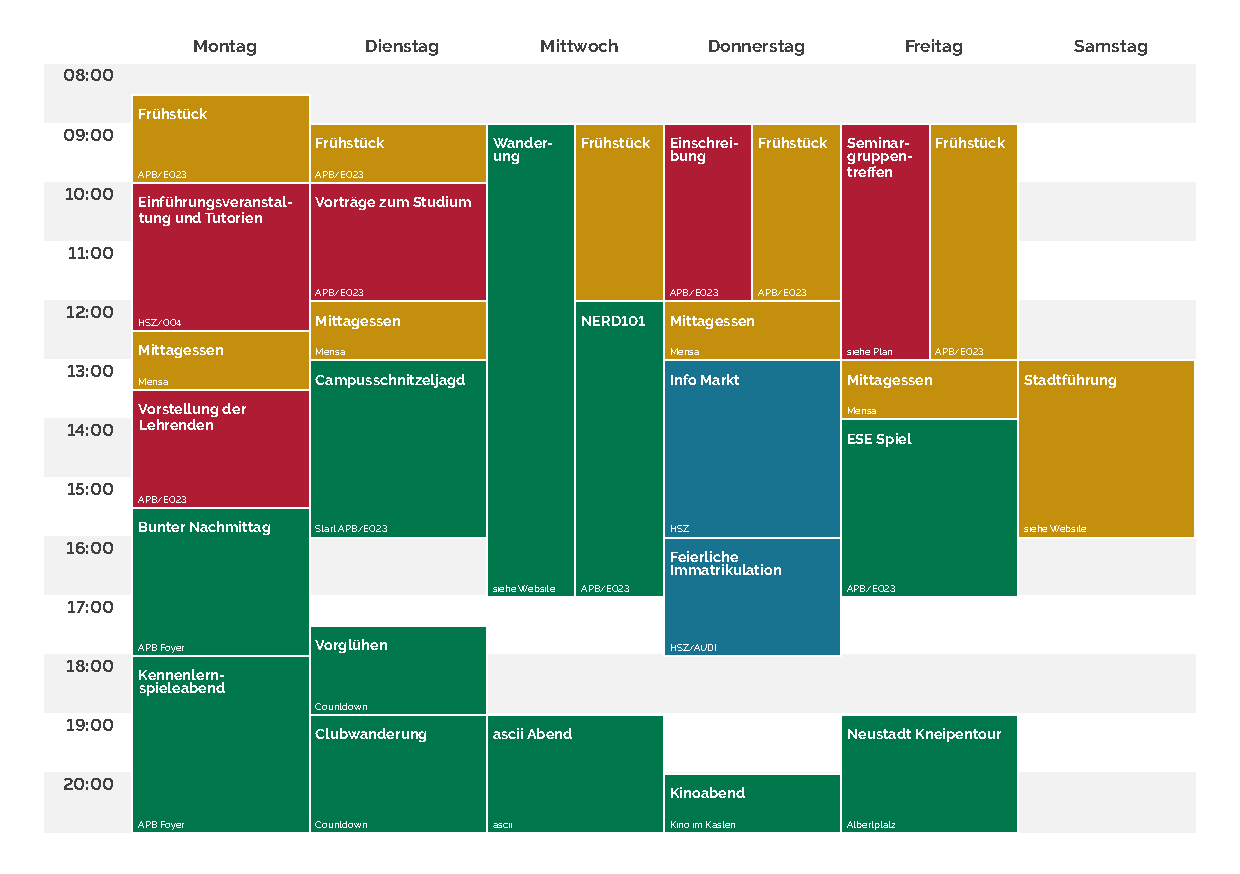
\includepdf[angle=90]{zeitplan_2019.pdf};
\end{document}

